\documentclass[conference]{IEEEtran}
\IEEEoverridecommandlockouts
% The preceding line is only needed to identify funding in the first footnote. If that is unneeded, please comment it out.
\usepackage{cite}
\usepackage{amsmath,amssymb,amsfonts}
\usepackage{algorithmic}
\usepackage{graphicx}
\usepackage{textcomp}
\usepackage{xcolor}
\usepackage[brazilian]{babel}
\usepackage[utf8]{inputenc}
\usepackage[T1]{fontenc}
\usepackage{listings}
\usepackage{color}
\usepackage{float}
\usepackage{multirow}
\usepackage{hyperref}

\definecolor{dkgreen}{rgb}{0,0.6,0}
\definecolor{gray}{rgb}{0.5,0.5,0.5}
\definecolor{mauve}{rgb}{0.58,0,0.82}

\lstset{frame=tb,
  language=Java,
  aboveskip=3mm,
  belowskip=3mm,
  showstringspaces=false,
  columns=flexible,
  basicstyle={\small\ttfamily},
  numbers=none,
  numberstyle=\tiny\color{gray},
  keywordstyle=\color{blue},
  commentstyle=\color{dkgreen},
  stringstyle=\color{mauve},
  breaklines=true,
  breakatwhitespace=true,
  tabsize=3
}
\lstset{language=Python}
\def\BibTeX{{\rm B\kern-.05em{\sc i\kern-.025em b}\kern-.08em
    T\kern-.1667em\lower.7ex\hbox{E}\kern-.125emX}}
\begin{document}

\title{Relatório do Laboratório 1: \\ File Transfer Protocol (FTP)\\
}

\author{\IEEEauthorblockN{Isabelle Ferreira de Oliveira}
\IEEEauthorblockA{\textit{CES-35 - Engenharia da Computação 2020} \\
\textit{Instituto Tecnológico de Aeronáutica (ITA)}\\
São José dos Campos, Brasil \\
isabelle.ferreira3000@gmail.com}
}

\maketitle

\begin{abstract}
O trabalho tem como objetivo a implementação de um servidor de transferência de arquivos básico inspirado na interface do File Transfer Protocol (FTP), com os requisitos conforme apresentados no roteiro do laboratório.
\end{abstract}

\begin{IEEEkeywords}
FTP, Redes de computadores, Cliente-Servidor
\end{IEEEkeywords}

\section{Implementação}\label{implementacao}

A linguagem de programação utilizada foi Python 3, com o auxílio das bibliotecas: \textit{socket} para comunicação entre os processos, \textit{thread} para a criação das threads para cada cliente conectado ao servidor, e \textit{shutil} e \textit{os} para os comandos de manipulação de diretórios e arquivos.

O código do Servidor pode ser simplificadamente explicado como a seguir. Ele se trata, inicialmente, de um loop infinito esperando tentativas de conexões advindas de clientes. Cada tentativa de conexão inicia uma thread que lida com cada sessão em particular. Ao chegar essa tentativa de conexão, o servidor começa, então, o processo de autenticação do cliente. Se o cliente fornecer corretamente seu nome de usuário e senha, inicia-se, por fim, outro loop infinito, dessa vez a espera de comandos digitados pelos usuários nos processos clientes. Caso o cliente falhe em sua antenticação, a conexão é encerrada. Cada comando que chega é devidamente lidado de acordo com suas peculiaridades.

Já o código do Cliente, de forma superficial, trata-se de um loop infinito esperando comandos advindos do usuário. Caso esteja conectado ao servidor, cada linha de comando é enviado para o servidor e ambos os processos passam a lidar com os resultados esperados. Caso esteja desconectado, o cliente é incapaz de realizar qualquer comando, exceto pelo de conectar-se ao servidor (comando \textit{open <server>}). Ao tentar se conectar ao servidor, o usuário é requisitado de digitar o nome de usuário e senha, para ocorrer a autenticação por parte do servidor.

Como cada comando é implementado, além de outras funcionalidades auxiliares foram melhores abordados nas subsessões a seguir.

\subsection{Funções auxiliares}

Cada mensagem trocada pelo cliente e servidor é recebida através da função a seguir. Essa função recebe a mensagem em pacotes de tamanho 16, concatenando-os para formar a mensagem completa. O fim da mensagem é identificado a partir de um \textit{carriage return} e \textit{line feed}.

\begin{lstlisting}
# Server and Client code
def receive_message(conn):
    message_received = ""
    while True:
        data_received = conn.recv(16)
        message_received = message_received + data_received.decode("utf-8")
        if message_received.endswith("\r\n"):
            break
    message_received = message_received.split("\r\n")[0]
    return message_received
\end{lstlisting}

A autenticação realizada no servidor foi apresentada a seguir. Ela se resume a comparação dos dados fornecidos pelo cliente aos armazenados em um mapa com nomes de usuários e senhas. Esse mapa é construído a partir da leitura de um arquivo de credenciais, e seu código também é apresentado a seguir.

\begin{lstlisting}
# Server code
def check_authentication(conn):
	conn.sendall(bytes("user:\r\n", 'utf-8'))
	username = receive_message(conn)

	conn.sendall(bytes("password:\r\n", 'utf-8'))
	password = receive_message(conn)
	
	authenticate = False
	if username in credentials:
		if credentials[username] == password:
			authenticate = True

	return authenticate, username
\end{lstlisting}

\begin{lstlisting}
# Server code
def create_credentials():
	credentials_file = open("credentials.txt", "r")
	lines = credentials_file.readlines()
	for line in lines:
		username = line.split(" ")[0]
		password = line.split(" ")[1]
		password = password.split("\n")[0]
		credentials[username] = password
\end{lstlisting}

As linhas de comando são digitadas pelo usuário no código do cliente, e essas linhas também são enviadas ao servidor. O parseamento dos comandos para serem lidados posteriormente são feitos através da função \textit{split} do Python, e teve seu código apresentado a seguir. 

\begin{lstlisting}
# Server and Client code
command = command_line.split(" ")[0]
args = command_line.split(" ")[1:]
\end{lstlisting}

\subsection{Navegação e listagem de diretórios}

Uma breve explicação de cada comando e a apresentação de sua implementação foram apresentados a seguir.

\subsubsection{cd <dirname>} Bastou concatenar o argumento \textit{dirname} ao path atual do cliente e, em seguida, utilizar a função \textit{os.chdir()} para mudar o diretório. Após isso, atualizar o path atual do cliente. Colocar também um \textit{try except} para conseguir um feedback de erro, como por exemplo, diretório inexistente no servidor.

\begin{lstlisting}
# Server code
if comm == "cd":
	curr_path = curr_session.current_directory

	try:
	    os.chdir(curr_path + "/" + dirname)
	    curr_path = os.getcwd()
	    curr_session.current_directory = curr_path
	    conn.sendall(bytes("ok\r\n", 'utf-8'))

	except FileNotFoundError:
	    conn.sendall(bytes("Error: directory does not exists in server \r\n", 'utf-8'))
\end{lstlisting}

\subsubsection{ls [dirname]} Bastou utilizar o comando \textit{os.listdir(path)} para obter a lista de arquivos e diretórios. Caso não venha com argumento dirname, path se trata do path atual do cliente; caso contrário, path se trata da concatenação do dirname ao path atual do cliente.

\begin{lstlisting}
# Server code
elif comm == "ls":
	if len(args) != 0:
	    dirname = args[0]
	    
	    try:
	    	path = curr_session.current_directory + "/" + dirname
	    	fileslist = os.listdir(path)
			conn.sendall(bytes(str(fileslist) + "\r\n", 'utf-8'))

	    except FileNotFoundError:
			conn.sendall(bytes("Error: directory does not exists in server\r\n", 'utf-8'))
	else:
		path = curr_session.current_directory
		fileslist = os.listdir(path)
	    conn.sendall(bytes(str(fileslist) + "\r\n", 'utf-8'))
\end{lstlisting}

\subsubsection{pwd} Bastou retornar o path atual do cliente.

\begin{lstlisting}
# Server code
elif comm == "pwd":
	path = curr_session.current_directory
	conn.sendall(bytes(path + "\r\n", 'utf-8'))
\end{lstlisting}

\subsection{Manipulação de diretórios}

\subsubsection{mkdir <dirname>} Bastou-se utilizar a função \textit{os.mkdir()}. Colocou-se também um \textit{try except} para conseguir um feedback de erro, como por exemplo, diretório já existente no servidor.

\begin{lstlisting}
# Server code
elif comm == "mkdir":
	try:
		path = curr_session.current_directory
	    os.mkdir(path + "/" + dirname)
	    conn.sendall(bytes("ok\r\n", 'utf-8'))

	except OSError:
	    conn.sendall(bytes("Error: directory already exists in server\r\n", 'utf-8'))
\end{lstlisting}

\subsubsection{rmdir <dirname>} Bastou-se utilizar a função \textit{shutil.rmtree()}. Colocou-se também um \textit{try except} para conseguir um feedback de erro, como por exemplo, diretório não existente no servidor.

\begin{lstlisting}
# Server code
elif comm == "rmdir":
	try:
		path = curr_session.current_directory
	    shutil.rmtree(path + "/" + dirname)
	    conn.sendall(bytes("ok\r\n", 'utf-8'))
	
	except OSError:
	    conn.sendall(bytes("Error: directory does not exists in server\r\n", 'utf-8'))
\end{lstlisting}

\subsection{Manipulação de arquivos}

\subsubsection{get <filename>} O comando \textit{get} foi mais complexo, principalmente devido a todas as verificações necessárias. Primeiro verificou-se a existência do arquivo no servidor. Em seguida, verificou-se a existência do arquivo no cliente. Caso tudo estivesse certo (ou seja, arquivo existente no servidor e inexistente no cliente), a transferência era realizada. A tranferência se tratava da leitura do arquivo em binário no servidor, do envio desse arquivo em pacotes de 1024 bytes para o cliente, que os recebia e escrevia em outro arquivo, também em binário. Caso o arquivo já existisse no cliente, era necessário também pedir a confirmação do usuário.

\begin{lstlisting}
# Server code
elif comm == "get":
	if check_if_file_exists(conn, filename):
		# if file not exists in local
		# or if can overwrite
	    feedback = receive_message(conn)

	    if feedback == "can get":
			path = curr_session.current_directory
			file = open(path + "/" + filename, "rb")
			aux = file.read(1024)
			while aux:
		    	conn.send(aux)
		    	aux = file.read(1024)
			conn.sendall(bytes("\r\n", 'utf-8'))
\end{lstlisting}

\begin{lstlisting}
# Client code
elif command == "get":
	# if file exists in server
	feedback = receive_message(sock)

	if feedback == "file already exists":
		# if file exists in local
		already_exists = check_if_file_already_exists(filename)

		can_get = True
		if already_exists:
			print("File already exists. Do you want to overwrite local file? [Y/N]")
			while True:
				answer = input()
				if answer.upper() == "Y":
					break
				elif answer.upper() == "N":
					can_get = False
					break
				else:
					print("Invalid answer. Please, answer with Y or N.")

		if can_get:
			sock.sendall(bytes("can get\r\n", 'utf-8'))
			f = open(str(filename), 'wb')
			aux = sock.recv(1024)
			while aux:
				f.write(aux)
				aux = sock.recv(1024)
				if aux.endswith(bytes("\r\n", 'utf-8')):
					break
			print("File downloaded!")
		else:
			sock.sendall(bytes("can not get\r\n", 'utf-8'))

	else:
		print("Error: file does not exists in server")
\end{lstlisting}

\subsubsection{put <filename>} O comando \textit{put} também foi mais complexo, devido a todas as verificações necessárias. Primeiro verificou-se a existência do arquivo no cliente. Em seguida, verificou-se a existência do arquivo no servidor. Caso tudo estivesse certo (ou seja, arquivo inexistente no servidor e existente no cliente), a transferência era realizada. A tranferência se tratava da leitura do arquivo em binário no cliente, do envio desse arquivo em pacotes de 1024 bytes para o servidor, que os recebia e escrevia em outro arquivo, também em binário. Caso o arquivo já existisse no servidor, era necessário também pedir a confirmação do usuário.

\begin{lstlisting}
# Server code
elif comm == "put":
	# if file exists in local
	feedback = receive_message(conn)

	if feedback == "files exists in local":
	    filename = filename.split("/")[-1]
	    
	    # if file exists in server
	    check_if_file_already_exists(conn, filename)

	    can_continue = receive_message(conn)
	    if can_continue == "Y":
	    	path = curr_session.current_directory
			f = open(path + "/" + filename, 'wb')
			aux = conn.recv(1024)
			while aux:
		    	f.write(aux)
		    	aux = conn.recv(1024)
		    	if aux.endswith(bytes("\r\n", 'utf-8')):
		        	break
		else:
			conn.sendall(bytes("ok\r\n", 'utf-8'))
\end{lstlisting}

\begin{lstlisting}
# Client code
elif command == "put":
	# if file exists in local
	file_exists_in_local = check_if_file_exists(filename)

	if file_exists_in_local:
		sock.sendall(bytes("files exists in local\r\n", 'utf-8'))
		
		# if file exists in server
		feedback = receive_message(sock)
		can_receive = False

		if feedback == "file already exists":
			print("File already exists. Do you want to overwrite remote file? [Y/N]")
			while True:
				answer = input()
				if answer.upper() == "Y":
					sock.sendall(bytes("Y\r\n", 'utf-8'))
					can_receive = True
					break
				elif answer.upper() == "N":
					sock.sendall(bytes("N\r\n", 'utf-8'))
					break
				else:
					print("Invalid answer. Please, answer with Y or N.")
		else:
			can_receive = True
			sock.sendall(bytes("Y\r\n", 'utf-8'))

		if can_receive:
			file = open(filename, "rb")
			aux = file.read(1024)
			while aux:
				sock.send(aux)
				aux = file.read(1024)
				sock.sendall(bytes("\r\n", 'utf-8'))
			print("File sent!")

	else:
		sock.sendall(bytes("files does not exists in local\r\n", 'utf-8'))
\end{lstlisting}

\subsubsection{delete <filename>} Bastou-se utilizar a função \textit{os.remove()}. Colocou-se também um \textit{try except} para conseguir um feedback de erro, como por exemplo, arquivo não existente no servidor.

\begin{lstlisting}
# Server code
elif comm == "delete":
	try:
		path = curr_session.current_directory
	    os.remove(path + "/" + filename)
	    conn.sendall(bytes("ok\r\n", 'utf-8'))

	except OSError:
	    conn.sendall(bytes("Error: file does not exists in server\r\n", 'utf-8'))
\end{lstlisting}

\subsection{Gerenciamento de conexões}

\subsubsection{close} Bastou-se utilizar a função \textit{conn.close()} tanto no servidor quanto no cliente. Além disso, era apagado o registro dessa conexão do mapa de sessões gerenciado pelo servidor.

\subsubsection{open <server>} O comando já foi bastante explicado nos segundo e terceiro parágrafos da sessão Implementação \ref{implementacao}. Pode-se acrescentar: o comando \textit{open} no servidor inicia a thread que lidará com o cliente, iniciado pela autenticação; no cliente, o comando \textit{open} inicia a conexão com o servidor, seguida da autenticação e do posterior loop inifinito a espera de linhas de comando. 

\subsubsection{quit} Bastou-se utilizar a função \textit{conn.close()} tanto no servidor quanto no cliente. Além disso, era apagado o registro dessa conexão do mapa de sessões gerenciado pelo servidor, e o processo do cliente era encerrado.

\begin{lstlisting}
# Server code
if command == "close" or command == "quit":
	sessions.pop(conn)
	conn.close()
	break
\end{lstlisting}

\section{Comentários adicionais}

Acerca das demais informações requisitadas para esse relatório, temos a seguir:

\begin{itemize}
\item O formato das mensagens enviadas pode ser visto tanto nos código apresentados acima, quanto nos diagramas de sequência apresentados na sessão a seguir. Esses diagramas de sequência foram apresentados nas Figuras de \ref{cd} a \ref{quit}. 

\item Já a estratégia utilizada para gerenciamento de conexões foram as threads individuais por sessão do cliente.

\item O próprio Python abstrai para o programador a alocação de memória para os comandos que envolvem envio e recebimento de arquivos (ou seja, \textit{get} e \textit{put}).

\item O parser de comandos no cliente foi apresentado nos códigos da sessão anterior, assim como aresolução de comandos no servidor.

\item As Figuras de \ref{cd1} a \ref{quit1} apresentam o correto funcionamento do código implementado, além de outras imagens anexadas a esse relatório.

\end{itemize}

\section*{Diagramas de Sequência}

\begin{figure}[H]
\centering
\centerline{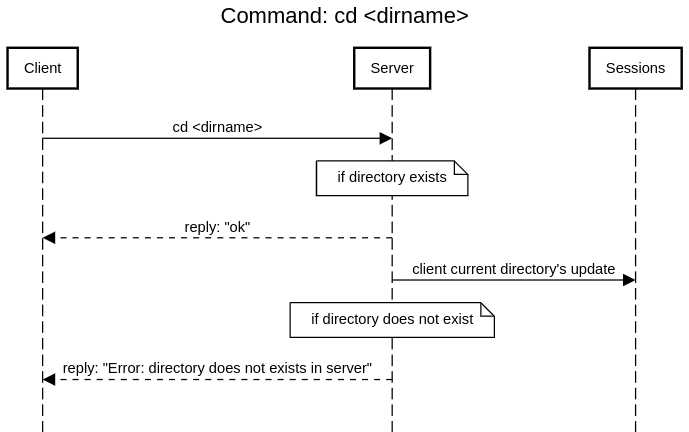
\includegraphics[scale=0.3]{diagrams/Command_cd_dirname.png}}
\caption{Diagrama de sequência do comando \textit{cd <dirname>}.}.
\label{cd}
\end{figure}

\begin{figure}[H]
\centering
\centerline{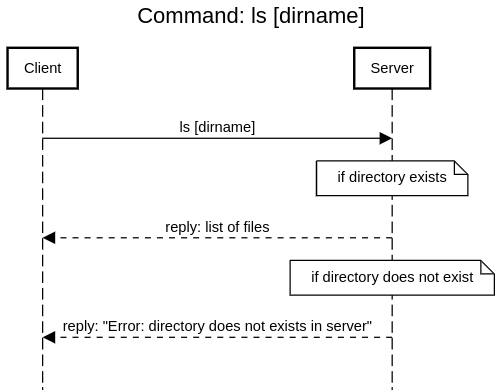
\includegraphics[scale=0.4]{diagrams/Command_ls_dirname.png}}
\caption{Diagrama de sequência do comando \textit{ls [dirname]}.}.
\label{ls}
\end{figure}

\begin{figure}[H]
\centering
\centerline{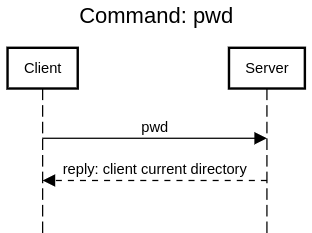
\includegraphics[scale=0.4]{diagrams/Command_pwd.png}}
\caption{Diagrama de sequência do comando \textit{pwd}.}.
\label{pwd}
\end{figure}

\begin{figure}[H]
\centering
\centerline{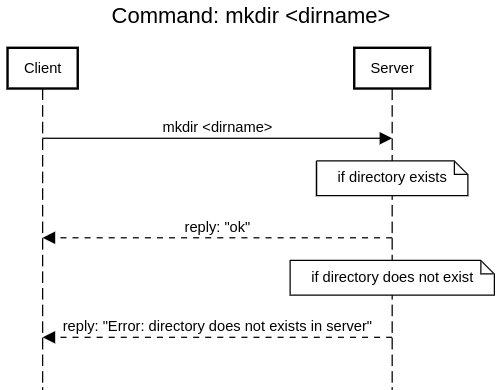
\includegraphics[scale=0.4]{diagrams/Command_mkdir_dirname.png}}
\caption{Diagrama de sequência do comando \textit{mkdir <dirname>}.}.
\label{mkdir}
\end{figure}

\begin{figure}[H]
\centering
\centerline{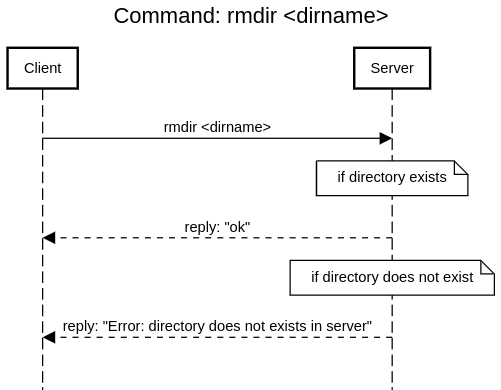
\includegraphics[scale=0.4]{diagrams/Command_rmdir_dirname.png}}
\caption{Diagrama de sequência do comando \textit{rmdir <dirname>}.}.
\label{rmdir}
\end{figure}

\begin{figure}[H]
\centering
\centerline{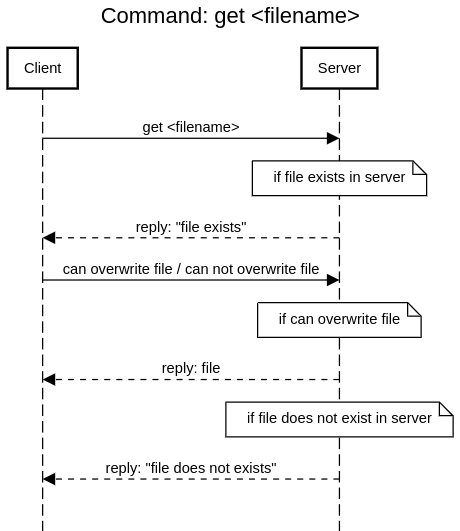
\includegraphics[scale=0.4]{diagrams/Command_get_filename.png}}
\caption{Diagrama de sequência do comando \textit{get <filename>}.}.
\label{get}
\end{figure}

\begin{figure}[H]
\centering
\centerline{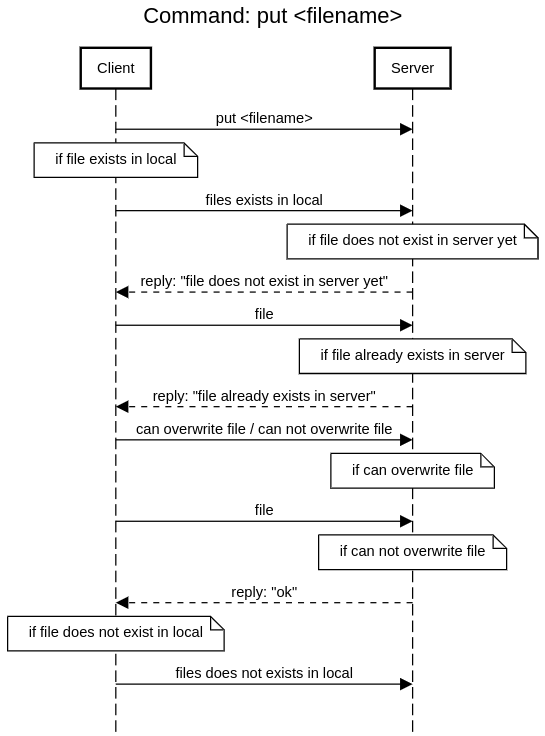
\includegraphics[scale=0.4]{diagrams/Command_put_filename.png}}
\caption{Diagrama de sequência do comando \textit{put <filename>}.}.
\label{put}
\end{figure}

\begin{figure}[H]
\centering
\centerline{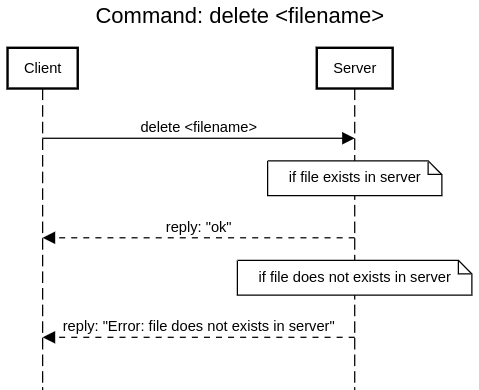
\includegraphics[scale=0.4]{diagrams/Command_delete_filename.png}}
\caption{Diagrama de sequência do comando \textit{delete <dirname>}.}.
\label{delete}
\end{figure}

\begin{figure}[H]
\centering
\centerline{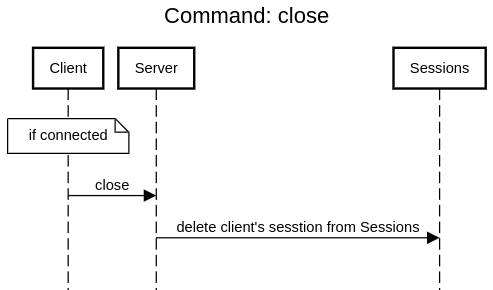
\includegraphics[scale=0.4]{diagrams/Command_close.png}}
\caption{Diagrama de sequência do comando \textit{close}.}.
\label{close}
\end{figure}

\begin{figure}[H]
\centering
\centerline{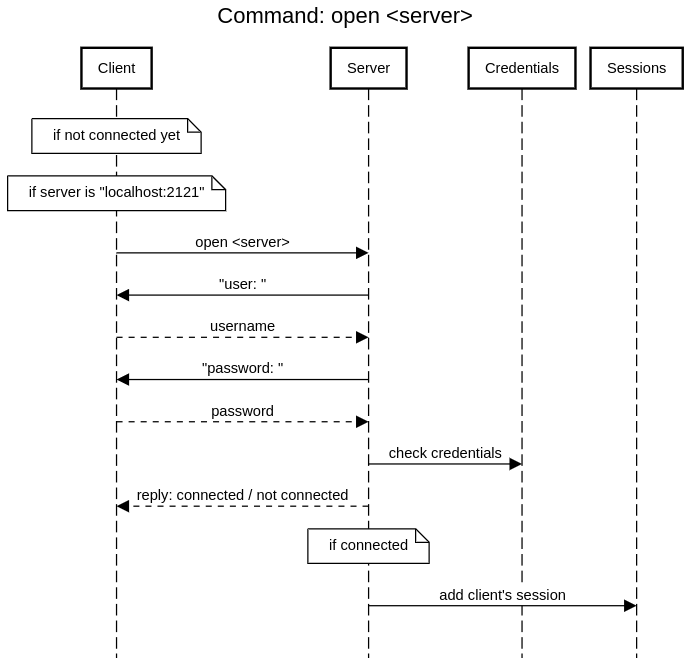
\includegraphics[scale=0.4]{diagrams/Command_open_server.png}}
\caption{Diagrama de sequência do comando \textit{open <server>}.}.
\label{open}
\end{figure}

\begin{figure}[H]
\centering
\centerline{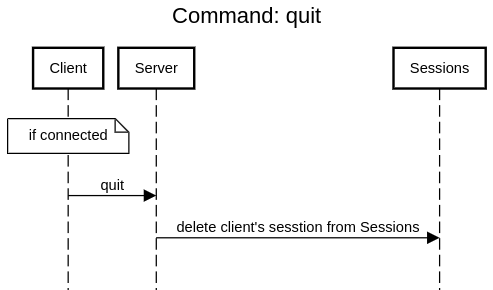
\includegraphics[scale=0.4]{diagrams/Command_quit.png}}
\caption{Diagrama de sequência do comando \textit{quit}.}.
\label{quit}
\end{figure}

\section*{Imagens do funcionamento}

\begin{figure}[H]
\centering
\centerline{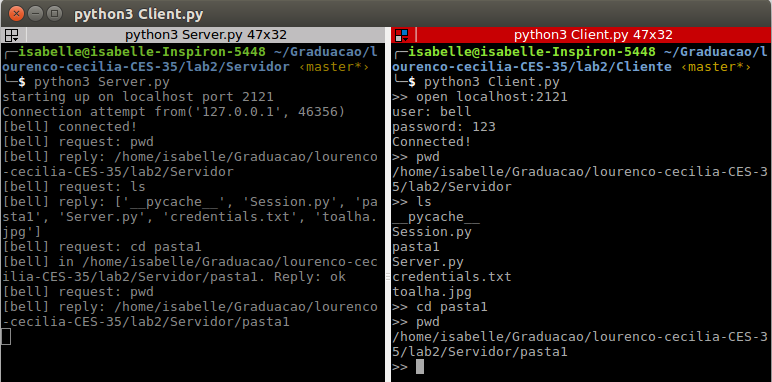
\includegraphics[scale=0.3]{prints/cd1.png}}
\caption{Funcionamento do comando \textit{cd <dirname>}.}.
\label{cd1}
\end{figure}

\begin{figure}[H]
\centering
\centerline{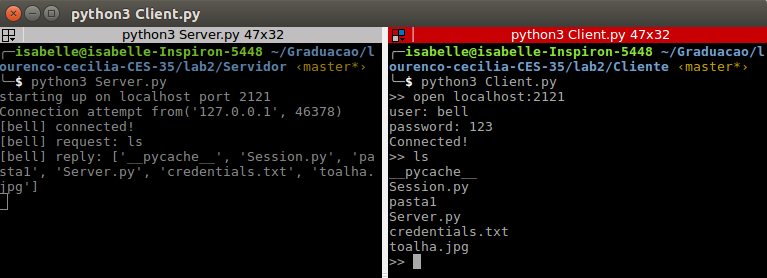
\includegraphics[scale=0.3]{prints/ls1.png}}
\caption{Funcionamento do comando \textit{ls [dirname]}.}.
\label{ls1}
\end{figure}

\begin{figure}[H]
\centering
\centerline{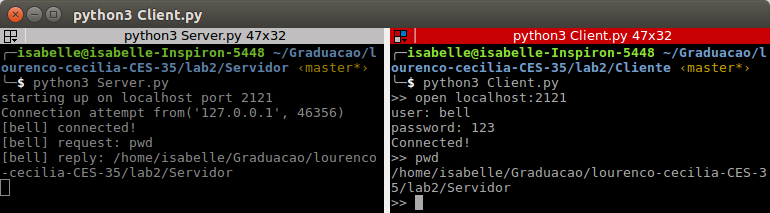
\includegraphics[scale=0.3]{prints/pwd.png}}
\caption{Funcionamento do comando \textit{pwd}.}.
\label{pwd1}
\end{figure}

\begin{figure}[H]
\centering
\centerline{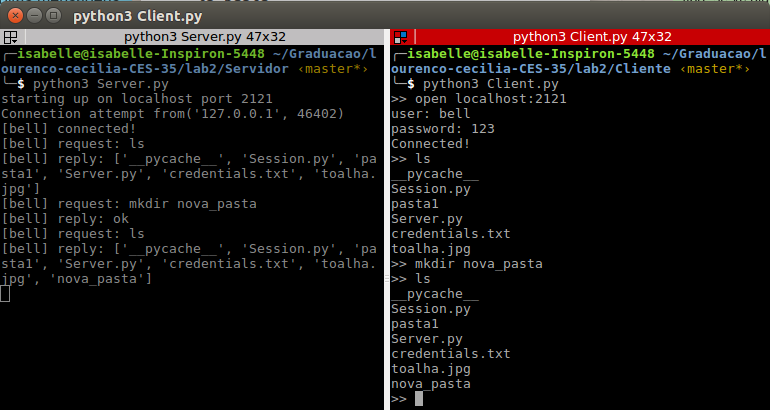
\includegraphics[scale=0.3]{prints/mkdir1.png}}
\caption{Funcionamento do comando \textit{mkdir <dirname>}.}.
\label{mkdir1}
\end{figure}

\begin{figure}[H]
\centering
\centerline{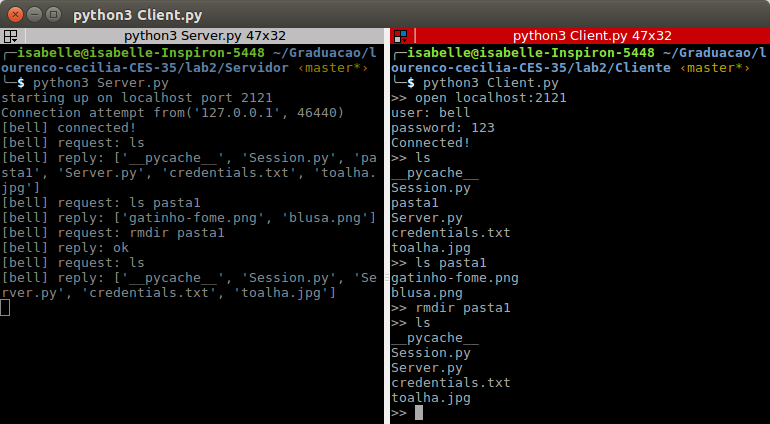
\includegraphics[scale=0.3]{prints/rmdir1.png}}
\caption{Funcionamento do comando \textit{rmdir <dirname>}.}.
\label{rmdir1}
\end{figure}

\begin{figure}[H]
\centering
\centerline{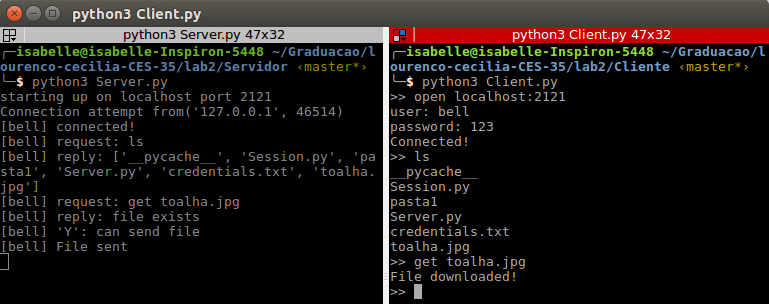
\includegraphics[scale=0.3]{prints/get1.png}}
\caption{Funcionamento do comando \textit{get <filename>}.}.
\label{get1}
\end{figure}

\begin{figure}[H]
\centering
\centerline{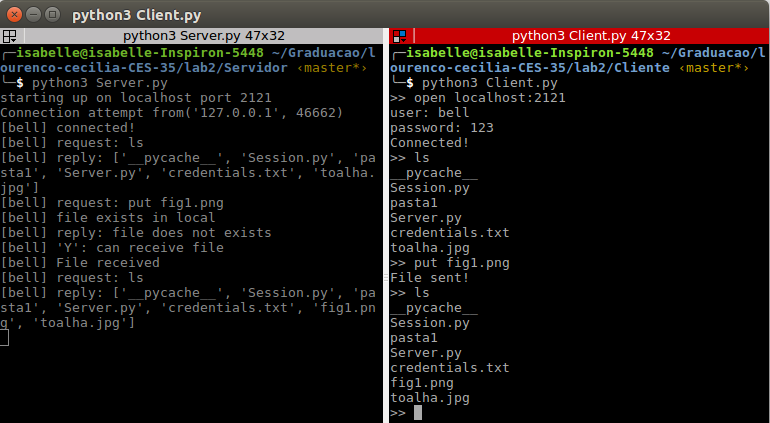
\includegraphics[scale=0.3]{prints/put1.png}}
\caption{Funcionamento do comando \textit{put <filename>}.}.
\label{put1}
\end{figure}

\begin{figure}[H]
\centering
\centerline{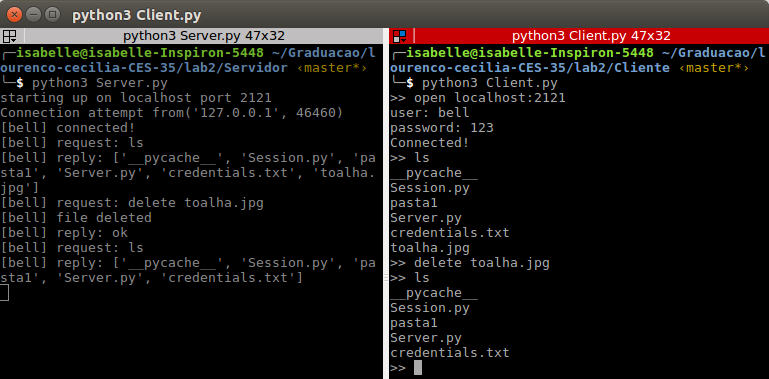
\includegraphics[scale=0.3]{prints/delete1.png}}
\caption{Funcionamento do comando \textit{delete <filename>}.}.
\label{delete1}
\end{figure}

\begin{figure}[H]
\centering
\centerline{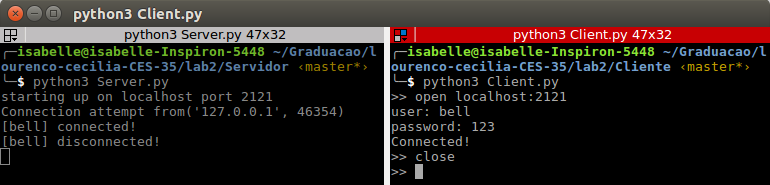
\includegraphics[scale=0.3]{prints/close.png}}
\caption{Funcionamento do comando \textit{close}.}.
\label{close1}
\end{figure}

\begin{figure}[H]
\centering
\centerline{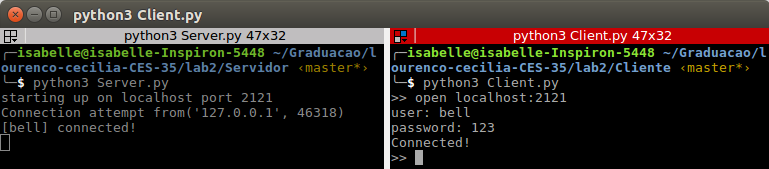
\includegraphics[scale=0.3]{prints/open1.png}}
\caption{Funcionamento do comando \textit{open <server>}.}.
\label{open1}
\end{figure}

\begin{figure}[H]
\centering
\centerline{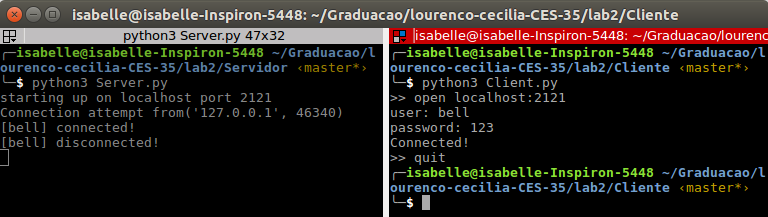
\includegraphics[scale=0.3]{prints/quit1.png}}
\caption{Funcionamento do comando \textit{quit}.}.
\label{quit1}
\end{figure}

\end{document}
